\documentclass[11pt]{article}
\usepackage[utf8]{inputenc}
\usepackage[T1]{fontenc}
\usepackage[margin = 2cm]{geometry}

\usepackage{palatino}
\usepackage{amsmath}
\usepackage{graphicx}
\usepackage{listings}
\usepackage{mathpazo}
\usepackage{hyperref}

\author{Samuele Bosi, Marco Ferrè, Philip Michael Grasselli, Simone Mariani}
\title{\textbf{CMLS Homework 1 – Audio Event Classification}}
\date{\today}

\begin{document}
\maketitle
\tableofcontents

\section{Introduction}
In this homework our task was to implement a classifier able to predict the audio event recorded in an audio excerpt.\\
In order to do this, we were provided with a collection of sampled sounds of a crowded urban area, each one corresponding to a given class among a group of 10. On the top of that, those audio files were also split into 10 different folders, and heterogeneously chosen with respect to the belonging classes.\\
Our main task was to analyze the different folders following precise criteria in order to create a model which -- for any chosen \textit{testing} folder -- recognizes for each file its belonging class, by means of performing tests on the signal characteristics along to some feature selection methods appropriately chosen by us.
All the work is pushed to GitHub on this following URL: \url{https://github.com/marcoferre/CMLS-HW1}.

\section{Analyzing the Data}

For this process, as suggested by the author of the sampled audio, we proceeded to apply a 10-fold cross-validation method: in a nutshell, this consists in selecting one fold for testing and using the remaining nine for training; after 10 iterations, corresponding to all possible combinations of testing folds, we get a pretty homogeneous analysis of the given data.\\
We chose to use the \textbf{MFCC (Mel-Frequency Cepstral Coefficient} as our main feature selection, where:
\begin{itemize}
\item all audio files are windowed by applying a Hamming window made of 1,024 samples, and a hop-size of 512 samples;
\item the STFT (Short-Time Fourier Transform) was computed for each audio file, and we ended up taking into consideration only the absolute values of the result;
\item we eventually created the \textbf{Mel filter}, with \texttt{n{\_}mels=40}, \texttt{f{\_}min=133.33} Hz, and \texttt{f{\_}max=6853.8} Hz, and we applied it to the modulus of the previously calculated STFT: all the computation is thus split into \texttt{n{\_}mfcc=13} blocks.
\end{itemize}

\begin{figure}
\centering
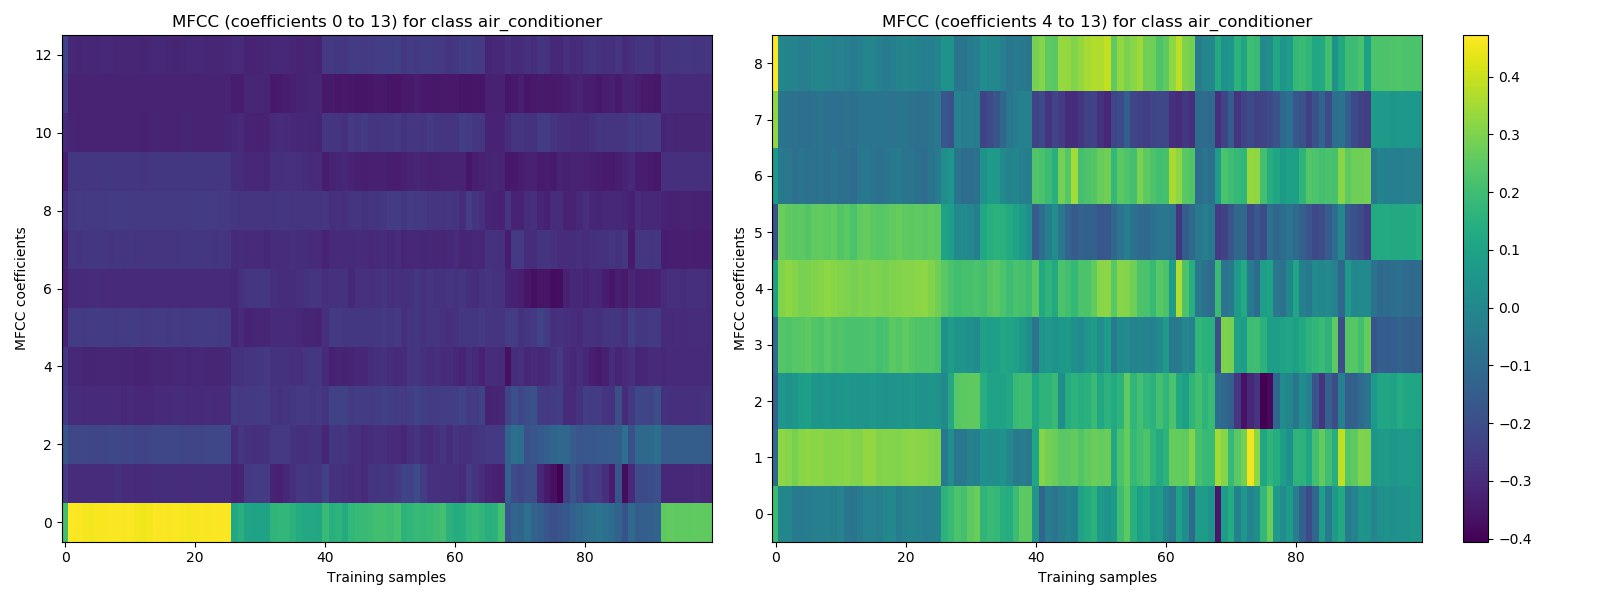
\includegraphics[width=1\textwidth]{AirCon}
\caption{The Air Conditioner MFC Coefficients}
\label{fig:AirCon}
\end{figure}

We appended all the obtained results for each audio file, belonging to each class, and enclosed in each fold, into a dictionary: for the class \texttt{air{\_}conditioner}, as an example, a representation is given in Figure \ref{fig:AirCon}.

\section{Classification by Means of Support Vector Machine (SVM)}
To perform the classification, we relied on the Support Vector Machine approach. Our final goal is to produce a \textbf{confusion matrix} for every iteration, where a different fold was taken as the test one.

\subsection{Motivation of the Features Choice}

\begin{figure}
\centering
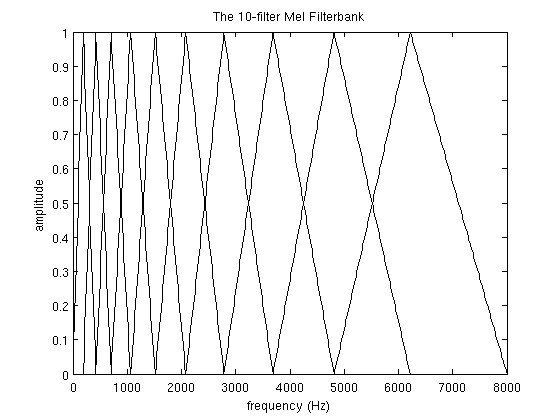
\includegraphics[width=0.5\textwidth]{A-Mel-filterbank-containing-10-filters}
\caption{The 10-Filter Mel Filterbank}
\label{fig:MFCC-graph}
\end{figure}

In the literature we can appreciate many different audio spectral descriptors, such as the Audio Spectrum Centroid, the Harmonic Ratio, etc. In our case, the Mel-Frequency Cepstrum Coefficients algorithm is the most appropriate for its accuracy in sampling the speech frequency band. This method is based on triangular filters whose center is placed accordingly to the \textbf{mel scale}, as shown in Figure \ref{fig:MFCC-graph}. For the sake of completeness, the following is the conversion formula of the frequency in Hertz in the mel scale:
\begin{equation}
\mathrm{Pitch} = 1127.0148\cdot \log\displaystyle\left(1+\frac{f}{700}\right)\mathrm{[mel]}
\end{equation}
Moreover, if we analyzed all the features, we would have a dramatic computational cost: we opted for a compromise in order to maintain the number of the considered test folds almost untouched. This is why we just considered only the MFCC as main parameter to pursue our task.

\subsection{The Dictionary}
In order to accomplish the first task, we initially created, for each fold, a \texttt{tot{\_}train{\_}features} dictionary, starting from the \texttt{tot{\_}features} calculated previously by removing from the latter one the features referring to the test fold of the corresponding iteration -- such that we have only the features linked to 9 folders of each of the 10 iterations.\\
Then, for each folder, we loaded into two vectors the feature values of each audio file, and we created four vectors divided by class:
\begin{itemize}
\item two of them would contain all the feature values for the training set, and the testing set, respectively, divided by class;
\item the other two would include the correct values to be associated to each element belonging to the relative class (e.g.: all the elements associated to the class \texttt{air{\_}conditioner} would have the 0 value, \texttt{car{\_}horn} elements would all have value 1, etc.). As for the two vectors previously itemized, we had also here one vector for the training set, and the other for the testing set. 
\end{itemize}

\subsection{Normalization}
We could calculate, in this phase, the maximum and the minimum values from all the training sets to perform the normalization process on the training and testing sets, which is needed to perform the SVM process without unbalances, as following:
\begin{equation}
\mathtt{X{\_}train{\_}normalized =  (X{\_}train - feat{\_}min) / (feat{\_}max - feat{\_}min)}
\end{equation}
\begin{equation}
\mathtt{X{\_}test{\_}normalized = (X{\_}test - feat{\_}min) / (feat{\_}max - feat{\_}min)}
\end{equation}

It is very important to underline the fact we used the same maximum and minimum values obtained from the training set also to normalize the testing set: this is done to ensure that, in a standard situation in which we didn't know which audio file would be given as input to the system, the model would be already created and it should have provided anyway appreciable results even for new and never-before-processed inputs.

\subsection{Exploiting the Support Vector Machine Classifier}
We, then, proceeded towards the actual classification by exploiting the \textbf{Support Vector Machine Classifier} taken from the \texttt{sklearn} library. Starting off, we created a $N\times N$ size dataframe using the \texttt{pandas} library (with $N$ being the number of the classes), that would fit the entire classification data of each one of the binary confrontation between the feature values of each class.\\
We filled this model by putting in the corresponding cell to the concatenation of the classes, taken by couples, the SVC fitting result of the concatenation of the normalized train elements of the two classes which are in analysis with the concatenation of the corresponding ideal output vectors of the same two ones. Then we append the result freshly obtained to the vector \texttt{y{\_}test{\_}predicted{\_}mc}, and normalizing the values between $-1$ and $1$.\\
Finally, we performed a majority voting in order to obtain the \texttt{y{\_}test{\_}predicted{\_}mv} vector, which we would use to calculate the multi-class confusion matrix for each one of the ten iterations. The call to this last method would provide also the \texttt{y{\_}test{\_}mc} vector, also known as the vector containing all the correct values that the process should have calculated during the classification process. The following is the confusion matrix referred to just the first fold, just as an example: on the main diagonal we have the correctly labeled values, the higher the better.

\begin{equation}
\begin{bmatrix}
63 & 0 & 0 & 0 & 2 & 6 & 0 & 5 & 7 & 17 \\
4 & 28 & 0 & 0 & 0 & 2 & 1 & 1 & 0 & 0 \\
14 & 0 & 36 & 0 & 12 & 14 & 13 & 5 & 1 & 5 \\
15 & 6 & 5 & 32 & 7 & 2 & 8 & 4 & 13 & 8 \\
1 & 5 & 19 & 0 & 60 & 2 & 7 & 4 & 0 & 2 \\
14 & 3 & 0 & 28 & 8 & 31 & 0 & 1 & 0 & 11 \\
0 & 0 & 0 & 2 & 8 & 1 & 22 & 1 & 0 & 1 \\
46 & 0 & 16 & 0 & 29 & 6 & 0 & 6 & 0 & 17 \\
1 & 0 & 4 & 11 & 0 & 4 & 1 & 0 & 60 & 5 \\
8 & 9 & 7 & 5 & 3 & 10 & 8 & 8 & 4 & 38
\end{bmatrix}
\end{equation}

\subsection{Final Results and Accuracy}
We eventually made a \textbf{confusion matrix} related to the accuracy related to all folds, with the percentage of samples recognized by our algorithm, rounded off to two decimals.

\begin{equation}
\begin{bmatrix}
21.5 & 0.7 & 16.1 & 3.2 & 4.6 & 1.9 & 1.8 & 23.7 & 3.3 & 23.2 \\
4.0 & 66.9 & 8.4 & 1.2 & 3.5 & 0.7 & 7.7 & 3.0 & 2.6 & 2.1 \\
4.9 & 1.8 & 42.8 & 5.2 & 7.0 & 3.8 & 13.6 & 7.8 & 2.5 & 10.6 \\
9.2 & 2.4 & 8.0 & 41.0 & 7.6 & 3.2 & 10.2 & 3.5 & 6.3 & 8.6 \\
6.9 & 3.6 & 7.2 & 5.9 & 32.9 & 4.8 & 8.9 & 24.7 & 1.7 & 3.4 \\
12.6 & 1.0 & 21.9 & 1.9 & 0.3 & 23.4 & 3.5 & 21.8 & 6.8 & 6.8 \\
1.3 & 1.9 & 10.4 & 2.9 & 12.3 & 2.1 & 54.8 & 7.5 & 0.8 & 5.9 \\
6.4 & 0.0 & 14.7 & 0.0 & 2.2 & 3.0 & 3.4 & 57.8 & 4.7 & 7.8 \\
8.7 & 1.7 & 5.0 & 10.8 & 0.5 & 3.5 & 4.0 & 0.9 & 63.0 & 2.0 \\
11.5 & 4.1 & 16.0 & 4.2 & 2.9 & 3.0 & 9.3 & 8.7 & 4.0 & 36.3
\end{bmatrix}
[\%]
\end{equation}
We gain the final accuracy by calculating the mean value of the main diagonal values:
\begin{equation}
\mathrm{Accuracy}=\frac{\displaystyle\sum_{i=0}^{9} \sum_{j=0}^{9} a_{ij}}{10}=44.0\% \qquad i=j
\end{equation}
\end{document}
